% url from which I found this template
% http://vision.stanford.edu/cs598_spring07/report_templates/

\documentclass[10pt,twocolumn,letterpaper]{article}

\usepackage{cvpr}
\usepackage{times}
\usepackage{epsfig}
\usepackage{graphicx}
\usepackage{amsmath}
\usepackage{amssymb}
\usepackage{subfigure}

% Include other packages here, before hyperref.

% If you comment hyperref and then uncomment it, you should delete
% egpaper.aux before re-running latex.  (Or just hit 'q' on the first latex
% run, let it finish, and you should be clear).
\usepackage[pagebackref=true,breaklinks=true,letterpaper=true,colorlinks,bookmarks=false]{hyperref}

\cvprfinalcopy % *** Uncomment this line for the final submission

\def\cvprPaperID{****} % *** Enter the CVPR Paper ID here
\def\httilde{\mbox{\tt\raisebox{-.5ex}{\symbol{126}}}}

% Pages are numbered in submission mode, and unnumbered in camera-ready
\ifcvprfinal\pagestyle{empty}\fi
\begin{document}

%%%%%%%%% TITLE
\title{\vspace{-2.0cm}Article Title}

\author{Francisco Camargo\\
Georgia Institute of Technology\\
%Institution1 address\\
{\tt\small fcamargo3@gatech.edu}
}

\maketitle

%%%%%%%%% ABSTRACT
\begin{abstract}
    In this work, we explore the robustness of Salvador's \etal~\cite{2019fb, fb_github} ingredient generating deep learning model given input images subject to adversarial perturbations. Blah blah blah blah blah blah blah blah blah blah. Blah blah blah blah blah blah blah blah blah blah. Blah blah blah blah blah blah blah blah blah blah.
\end{abstract}

%%%%%%%%% BODY TEXT
\section{Introduction}
Blah blah blah blah blah blah blah blah blah blah. Blah blah blah blah blah blah blah blah blah blah. Blah blah blah blah blah blah blah blah blah blah. Blah blah blah blah blah blah blah blah blah blah. Blah blah blah blah blah blah blah blah blah blah. Blah blah blah blah blah blah blah blah blah blah. Blah blah blah blah blah blah blah blah blah blah.

Blah blah blah blah blah blah blah blah blah blah.~\cite{BossardFood101, salvador2017learning, 2019fb}. Blah blah blah blah blah blah blah blah blah blah.~\cite{2019fb} Blah blah blah blah blah blah blah blah blah blah. Blah blah blah blah blah blah blah blah blah blah. Blah blah blah blah blah blah blah blah blah blah. Blah blah blah blah blah blah blah blah blah blah.

Blah blah blah blah blah blah blah blah blah blah. Blah blah blah blah blah blah blah blah blah blah. Blah blah blah blah blah blah blah blah blah blah. Blah blah blah blah blah blah blah blah blah blah. Blah blah blah blah blah blah blah blah blah blah.

\subsection{Related Work}
Blah blah blah blah blah blah blah blah blah bla~\cite{BossardFood101}. Blah blah blah blah blah blah blah blah blah blah~\cite{salvador2017learning}. Blah blah blah blah blah blah blah blah blah blah~\cite{marin2019learning}. Blah blah blah blah blah blah blah blah blah blah.Blah blah blah blah blah blah blah blah blah blah.Blah blah blah blah blah blah blah blah blah blah.

Blah blah blah blah blah blah blah blah blah blah~\cite{2019fb}. Blah blah blah blah blah blah blah blah blah blah~\cite{vaswani_attention_2017}. Blah blah blah blah blah blah blah blah blah blah. Blah blah blah blah blah blah blah blah blah blah. Blah blah blah blah blah blah blah blah blah blah. Blah blah blah blah blah blah blah blah blah blah. Blah blah blah blah blah blah blah blah blah blah.

Blah blah blah blah blah blah blah blah blah blah~\cite{2019fb} Blah blah blah blah blah blah blah blah blah blah. Blah blah blah blah blah blah blah blah blah blah. Blah blah blah blah blah blah blah blah blah blah. Blah blah blah blah blah blah blah blah blah blah. Blah blah blah blah blah blah blah blah blah blah. Blah blah blah blah blah blah blah blah blah blah.

\subsection{Data}
Blah blah blah blah blah blah blah blah blah blah~\cite{2019fb}. Blah blah blah blah blah blah blah blah blah blah~\ref{table:1}. Blah blah blah blah blah blah blah blah blah blah. Blah blah blah blah blah blah blah blah blah blah. Blah blah blah blah blah blah blah blah blah blah. Blah blah blah blah blah blah blah blah blah blah. Blah blah blah blah blah blah blah blah blah blah.

\begin{table}[h!]
\begin{center}
 \begin{tabular}{c c c} 
 \hline
 Partition & Images & Number of Recipes \\
 \hline
 Training & 252,547 & 720,639 \\ 
 Validation & 54,255 & 155,036 \\
 Test & 54,506 & 154,045 \\
 \hline
 Total & 361,308 & 1,029,720 \\
 \hline
\end{tabular}
\end{center}
\caption{Number of samples by partition for Recipe 1M Dataset.}
\label{table:1}
\end{table}

%------------------------------------------------------------------------
\section{Approach}
Blah blah blah blah blah blah blah blah blah blah~\cite{2019fb, fb_github}. Blah blah blah blah blah blah blah blah blah blah~\cite{he_deep_2016}. Blah blah blah blah blah blah blah blah blah blah. Blah blah blah blah blah blah blah blah blah blah. Blah blah blah blah blah blah blah blah blah blah. Blah blah blah blah blah blah blah blah blah blah. Blah blah blah blah blah blah blah blah blah blah. Blah blah blah blah blah blah blah blah blah blah. Blah blah blah blah blah blah blah blah blah blah. Blah blah blah blah blah blah blah blah blah blah. Blah blah blah blah blah blah blah blah blah blah. Blah blah blah blah blah blah blah blah blah blah.

Blah blah blah blah blah blah blah blah blah blah (fig.~\ref{fig:image_examples}). Blah blah blah blah blah blah blah blah blah blah. Blah blah blah blah blah blah blah blah blah blah. Blah blah blah blah blah blah blah blah blah blah. Blah blah blah blah blah blah blah blah blah blah. Blah blah blah blah blah blah blah blah blah blah. Blah blah blah blah blah blah blah blah blah blah. Blah blah blah blah blah blah blah blah blah blah.

\begin{itemize}
    \item \textbf{Gaussian Blur} using \texttt{OpenCV} library~\cite{OpenCV_blur}, this filter blurs an image by applying $n \times n $ sized kernel filter across the entire image. Higher the kernel size leads to more blurring effect. We modified the filter from 3x3 to 45x45.\\
    \item \textbf{Salt \& Pepper} ~\cite{gonzalez_digital_2008} applies image degradation by randomly updating the pixel values to be 0 or 255. Overall extent is controlled by the percentage of pixel on which the noise is applied. We modified the percentage from 1 percent to 90 percent.\\
    \item \textbf{Gaussian Noise} is a type of statistical noise that has a probability density function that's equivalent to the Gaussian distribution \[
  X \sim \mathcal{N}(\mu,\,\sigma^{2})\,.
\]   and is additive. We added noise with mean of 1 and variance of 1 to mean of 250 and variance of 50.\\
    \item \textbf{Poisson} applies a Poisson distributed noise across the image and is additive in nature.
    \[
   \frac{{e^{ - \lambda } \lambda ^x }}{{x!}}
\] Lambda was simulated from 1 to 50.\\
    \item \textbf{Speckle} noise is generated by taking random pixels and multiplying it with a random value. Overall extent is controlled by the percentage of pixel on which the noise is applied. Speckle percentage was simulated from 1 percent to 90 percent
    \item \textbf{Black \& White} noise is taking an input image and converting it to black and white. We tried the black and white image with various cutoffs, but eventually applied a cutoff at 127. This means that all the pixels with value less than 127 get updated to 0 and all pixels with value greater than 127 are converted to 255.
    \item \textbf{Style Transfer} following Gaty \etal~\cite{gatys_neural_2015} where a feature space generated by 16 convolutional and 5 pooling layers of a 19 layer VGG-Network can be used as an algorithm to create artistic images. We utilized the same style throughout the different sets of models by differentiating the content loss weight. The weight ratio of content weight to the style weight ranges from 0.9 to 5000. These images were generated using a GPU Tesla 4 equipped with 15GB of RAM.
\end{itemize}

\begin{figure}[h]
    \centering
    \subfigure[Original]{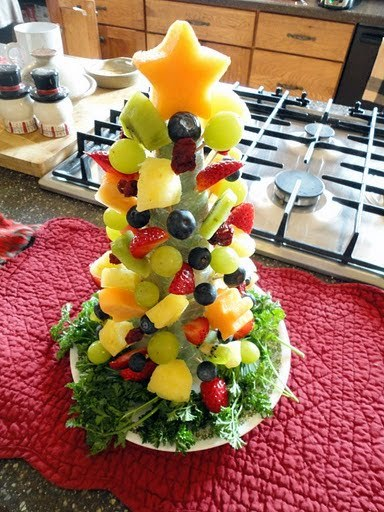
\includegraphics[width=0.15\textwidth]{images/22a3fb84d5_original.png}} 
    \subfigure[Gaussian Blur]{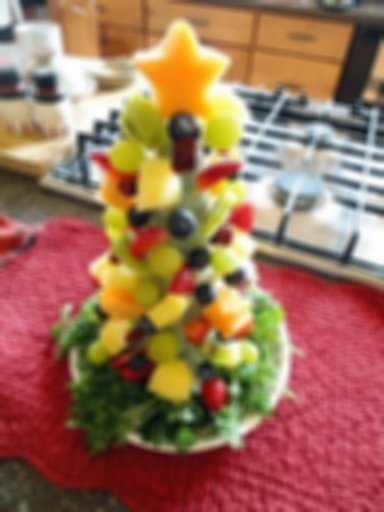
\includegraphics[width=0.15\textwidth]{images/22a3fb84d5_blurry_m5.png}} 
    \caption{Original image and image perturbations.}
    \label{fig:image_examples}
\end{figure}

Blah blah blah blah blah blah blah blah blah blah~\cite{chen_chinesefoodnet_2017}). Blah blah blah blah blah blah blah blah blah blah~\cite{salvador2017learning, 2019fb}. Blah blah blah blah blah blah blah blah blah blah~\cite{salvador2017learning, mit_github}. Blah blah blah blah blah blah blah blah blah blah. Blah blah blah blah blah blah blah blah blah blah. Blah blah blah blah blah blah blah blah blah blah. Blah blah blah blah blah blah blah blah blah blah. Blah blah blah blah blah blah blah blah blah blah. Blah blah blah blah blah blah blah blah blah blah.

\section{Experiment: Similarity Effects}
Blah blah blah blah blah blah blah blah blah blah~\cite{arandjelovic_three_2012}. Blah blah blah blah blah blah blah blah blah blah. Blah blah blah blah blah blah blah blah blah blah. Blah blah blah blah blah blah blah blah blah blah. Blah blah blah blah blah blah blah blah blah blah. Blah blah blah blah blah blah blah blah blah blah. Blah blah blah blah blah blah blah blah blah blah. Blah blah blah blah blah blah blah blah blah blah.

%-------------------------------------------------------------------------
{\small
\bibliographystyle{ieee_fullname}
\bibliography{egbib}
}

\end{document}